\input{style/settings}
\input{style/short_commands}
\pagestyle{fancy}
\fancyhf{}
\fancyhead[R]{página\;\thepage/\pageref{LastPage}}
\fancyhead[L]{Osvaldo Uriel Calderón Dorantes}
\fancyfoot[L]{Seguridad Radiológica}
\fancyfoot[R]{Facultad de Ciencias, UNAM 
\includegraphics[scale=0.13]{style/Sheikah.pdf}}
\fancypagestyle{plain}{
  \fancyfoot[C]{}
}
\makeatletter
\def\@seccntformat#1{%
  \expandafter\ifx\csname c@#1\endcsname\c@section\else
  \csname the#1\endcsname\quad
  \fi}
\makeatother
%%%%%%%%%%%%%%%%%%%%%%%%%%%%%%%%%%%%%%%%%%%%%%%%%%%%%%%
%%%%%%%%%%%%%%%%%%%%%%%%%%%%%%%%%%%%%%%%%%%%%%%%%%%%%%%%%%%
\begin{document}
\begin{flushleft}
Osvaldo Uriel Calderón Dorantes, \hfill Seguridad Radiológica\\
316005171 \hfill osvaldo13576@ciencias.unam  \\
Facultad de Ciencias\\
\underline{Universidad Nacional Autónoma de México}
\end{flushleft}

\begin{flushright}\vspace{-5mm}

\includegraphics[height=1.5cm]{style/logo.pdf}
\end{flushright}
 
\begin{center}\vspace{-1cm}
\textbf{ \large \customfont{Examen Parcial 1}}\\
\today
\end{center}
\medskip\hrule\medskip
%%%%%%%%%%%%%%%%%%%%%%%%%%%%%%%%%%%%%%%%%%%%%%%%


\newlength{\strutheight}
\settoheight{\strutheight}{\strut}
\begin{enumerate}
  \item ¿Existen las moléculas monoatómicas? Justifique.
  
  Aunque moléculas se pueden referir como elementos propiamente, hay elementos que son más abundantes en su forma diatómica como el hidrógeno el cual el par de hidrógenos están unidos por enlace covalente y esta unión es más estable.


  \item ¿Cuál es la notación utilizada para describir a un núcleo determinado? Sea explícito
  
\eq{e:p2}{^A_ZX_N}
La notación empleada para describir a un núcleo es la etiquetada en la ecuación \ref{e:p2}, donde \ec{Z} es el número atómico o número de protones, \ec{N} el número de neutrones \ec{A} es el número de masa \ec{A=Z+N} y \ec{X} es el nombre del átomo.

  \item ¿A que se refiere la ley del octeto?
  
Se refiere a que todo elemento tiende a formar enlace químicos (excepto el hidrógeno y helio) para obtener la misma configuración electrónica de un gas noble, tener los ocho electrones en su capa de valencia. 

  \item ¿Qué tipo de efectos se espera de la interacción electromagnética (radiación ionizante) con la materia, describa los 3 principales?
  
\begin{itemize}
  \item Efecto fotoeléctrico: Un fotón incide sobre un electrón de la capa interna del átomo y es absorbido completamente, esto hace que el electrón salga expulsado y deje una vacante para los electrones de las capas superiores externas.
  \item Efecto Comptom: Un fotón incide sobre los electrones de las capas superiores externas del átomo, no es absorbido completamente, sino que que el fotón sale expulsado un una diferente longitud de onda.
  \item Producción de pares: En esta interacción hay un fotón incidente cuya interacción produce un electrón y un positrón.
\end{itemize}


  \item ¿Cuáles son los dos elementos mas probables del cuerpo humano con los cuales interacciona los neutrones térmicos? Escribe la reacción nuclear.
  
Los elementos son  el nitrógeno y el hidrógeno, cuya reacción es

\dcasos{
  \tx{Nitrógeno:}& ^{14}N(n,p)\;^{14}C\\
  \tx{Hidrógeno:}& ^{1}H(n,\gamma)\;^{2}H
  }




  \item Defina radiosensibilidad y mencione en qué tipo de células se favorece.
  
La radiosensibilidad es la susceptibilidad de una célula o tejido a la radiación, las células radiosensibles son las que están continuamente replicándose, tienen una actividad metabólica aumentada o células de tejido joven o embrionario, como ejemplo tenemos a las células madre hematopoyéticas las cuales tienen diferentes rutas de diferenciación dando lugar a los glóbulos rojos y los glóbulos blancos.


  \item ¿Cuál es el alcance en aire para la partícula beta proveniente del 90Y?
  
  
Para este caso tenemos \ec{E_{\beta\tx{máx}}=2.2785[MeV]}

  \al{R_{\beta,\tx{aire}}(\;^{90}Y)&=\dfrac{412{E_{\beta\tx{máx}}}(\;^{90}Y)^{1.265-0.0954\ln(E_{\beta\tx{máx}}(\;^{90}Y))}}{\rho_m}\\
  &=\dfrac{412\cdot{2.2785}^{1.265-0.0954\ln(2.2785)}}{1.293}[cm]\\
  &=846.5[cm]
  }


  \item Describa el Síndrome Agudo de la Radiación.
  
Es una enfermedad causada por elevadas dosis de radiación, como síndrome lleva un conjunto de enfermedades asociadas en un corto periodo de tiempo, los cuales llevan problemas en la sangre o médula ósea (hematopoyético), problemas gastrointestinales y del sistema nervioso central.


  \item Mencione una fuente de neutrones y describa su funcionamiento.
  

  Fuente: Fuentes emisoras \ec{\alpha}, se bombardea con partículas ciertos blancos de ligeros cuyos productos resulta en un neutrón y otro elemento, por ejemplo:

\ecc{\alpha+\;^{9}_{4}Be\longrightarrow\;^{12}_{6}C+\;^{1}_{0}n}


  \item Escribe la configuración electrónica del 45Ca (emisor beta menos).
  
  \ecc{1s^2 \;2s^2 \;2p^6 3s^2 \;3p^6 \;4s^2}

  \item  Describe y dibuje como es el espectro de emisión del Ra-226, cuya alfa es de 4.8 MeV (considere una intensidad del 100\%).
  


  \item  ¿Qué tipo de valencia tiene el Aluminio y cuál es?
  
Tiene valencia de tipo positiva y es 3.


  \item  ¿Qué es el filtrado inherente en un tubo de rayos X?
  
Es un filtro que viene por sí mismo en la estructura del tubo de rayos X y consiste en una ventana de berilio y en el espectro elimina rayos X débiles.



  \item  ¿Cuál es alcance en aire de las partículas alfa proveniente del 225Ac, cuya energía máxima es de 5 MeV?
  
Tenemos que \ec{E_{\alpha\tx{máx}}(\;^{225}Ac=5[MeV])}

  \al{R_{\alpha,\tx{aire}}(\;^{225}Ac)&=1.24 \cdot E_{\alpha\tx{máx}}(\;^{225}Ac)-2.62\\
  &=1.24 \cdot 5-2.62\\
  &=3.58[cm]
  }


  \item  ¿Qué es el decaimiento radiactivo?
  
  Es la desintegración de un núcleo inestable a uno que es energéticamente más estable.


  \item  Escriba las ecuaciones de decaimiento de dos mecanismos ( alfa, beta+, beta- o captura electrónica) y la ecuación para obtener el valor Q de los mismos.
  

\begin{itemize}
  \item Decaimiento \ec{\alpha}:
  Se describe por la ecuación 
  \ecc{^A_Z X_N\longrightarrow\;^{A-4}_{Z-2}Y_{N-2}+\alpha}
  cuyo valor de Q es:
  \ecc{Q_\alpha=\p{m_X+m_Y-m_\alpha}c^2}
  \item Decaimiento \ec{\beta+}:
  Se describe por la ecuación
  \ecc{ ^A_Z X_N \longrightarrow\;^{A}_{Z-1}Y_{N+1}+\beta^+ +\nu}
  cuyo valor de Q es:
  \ecc{Q_{\beta^+}=\p{m(\;^AZ)-m(\;^A Y)-2m_e}c^2}

\end{itemize}


  \item  Dibuje un espectro de emisión de la partícula beta para el 64Cu y explique.
  



  \item  ¿Qué es la atenuación de los fotones y el endurecimiento del haz?
  
  El endurecimiento del haz se refiere a la pérdida, selectiva, de fotones de menor energía de un haz policromático con  filtro. Este efecto provoca que dé como resultado que haya un cambio en el espectro de rayos X, pero no de los picos de   energía máximas, aunque sí lo hace la energía promedio que hace que aumente (lo cual puede que genere artefactos en
  la imagen de TC), entonces, el concepto viene que el haz se vuelva más penetrante conforme aumente la energía promedio   de los fotones. 
  
  
  En cuanto a la atenuación de los fotones se refiere al cambio de intensidad cuando pasan por un medio, por la ley de la atenuación en un medio lineal se describe por la ecuación
  \ecc{I=I_0e^{-\mu x}}
donde \ec{I_0} es la intensidad de los fotones inicial, \ec{x} es el grosor del material y \ec{\mu} es el índice de atenuación lineal.

  \item  Explique el fenómeno de producción de pares, la condición para que ocurra y el destino final de los productos.
  

Es una reacción que ocurre cerca del núcleo atómico en donde incide un fotón crea un par de partículas: un electrón y un positrón, en donde el fotón debe tener una energía mayor a \ec{1.022 [MeV]}, las partículas creadas  pueden alejarse unas de otras si tienen suficiente energía cinética para escapar de la atracción electrostática




  \item  La siguiente gráfica corresponde al espectro generado por un tubo de rayos X, escriba el nombre de los ejes y las partes señaladas por las viñetas.
  

\begin{figure}[!ht]
\centering
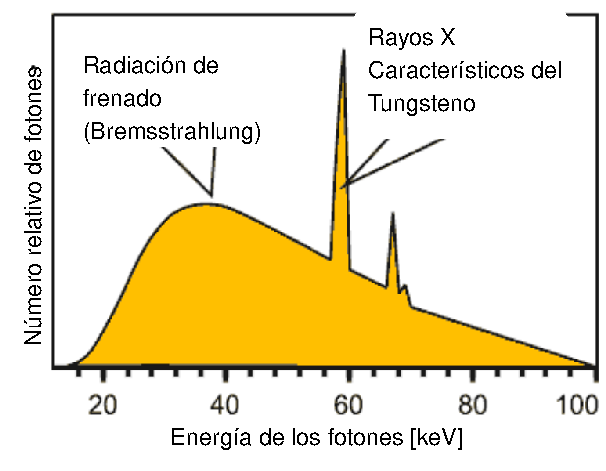
\includegraphics[width=0.4\textwidth]{./figuras/fig_p20_ex.pdf}
\caption{Espectro de emisión de un tubo de rayos X}
\label{fig:p20_ex}
\end{figure}

  \item  ¿Qué es la moderación de los neutrones, y cuáles son los neutrones térmicos?
  



\end{enumerate}

%\begin{multicols}{2}
%\small{\bibliographystyle{apalike}
%\bibliography{bib}}
%\end{multicols}



%\ftikz{1.5}{figuras/fig.tikz}{}{fig:x}

\end{document}



}